\documentclass[a4paper,kulak]{kulakarticle}

\usepackage[utf8]{inputenc}
\usepackage[dutch]{babel}
\usepackage{pdfpages}
\usepackage{subfig}
\usepackage{float}

\usepackage{cite}

% style
%\usepackage[left=2.5cm,top=2cm,right=2.5cm,bottom=2cm,a4paper]{geometry}
\usepackage{color}

\date{\today}
\address{
	Bachelor in de fysica\\
	Bachelor in de informatica\\
	Bachelor in de wiskunde\\
	Ingenieurswetenschappen}
\title{BDA App}
\author{Marthe B\"{o}ting\\
	Robin Bruneel\\
	Toon Ingelaere}

\begin{document}
	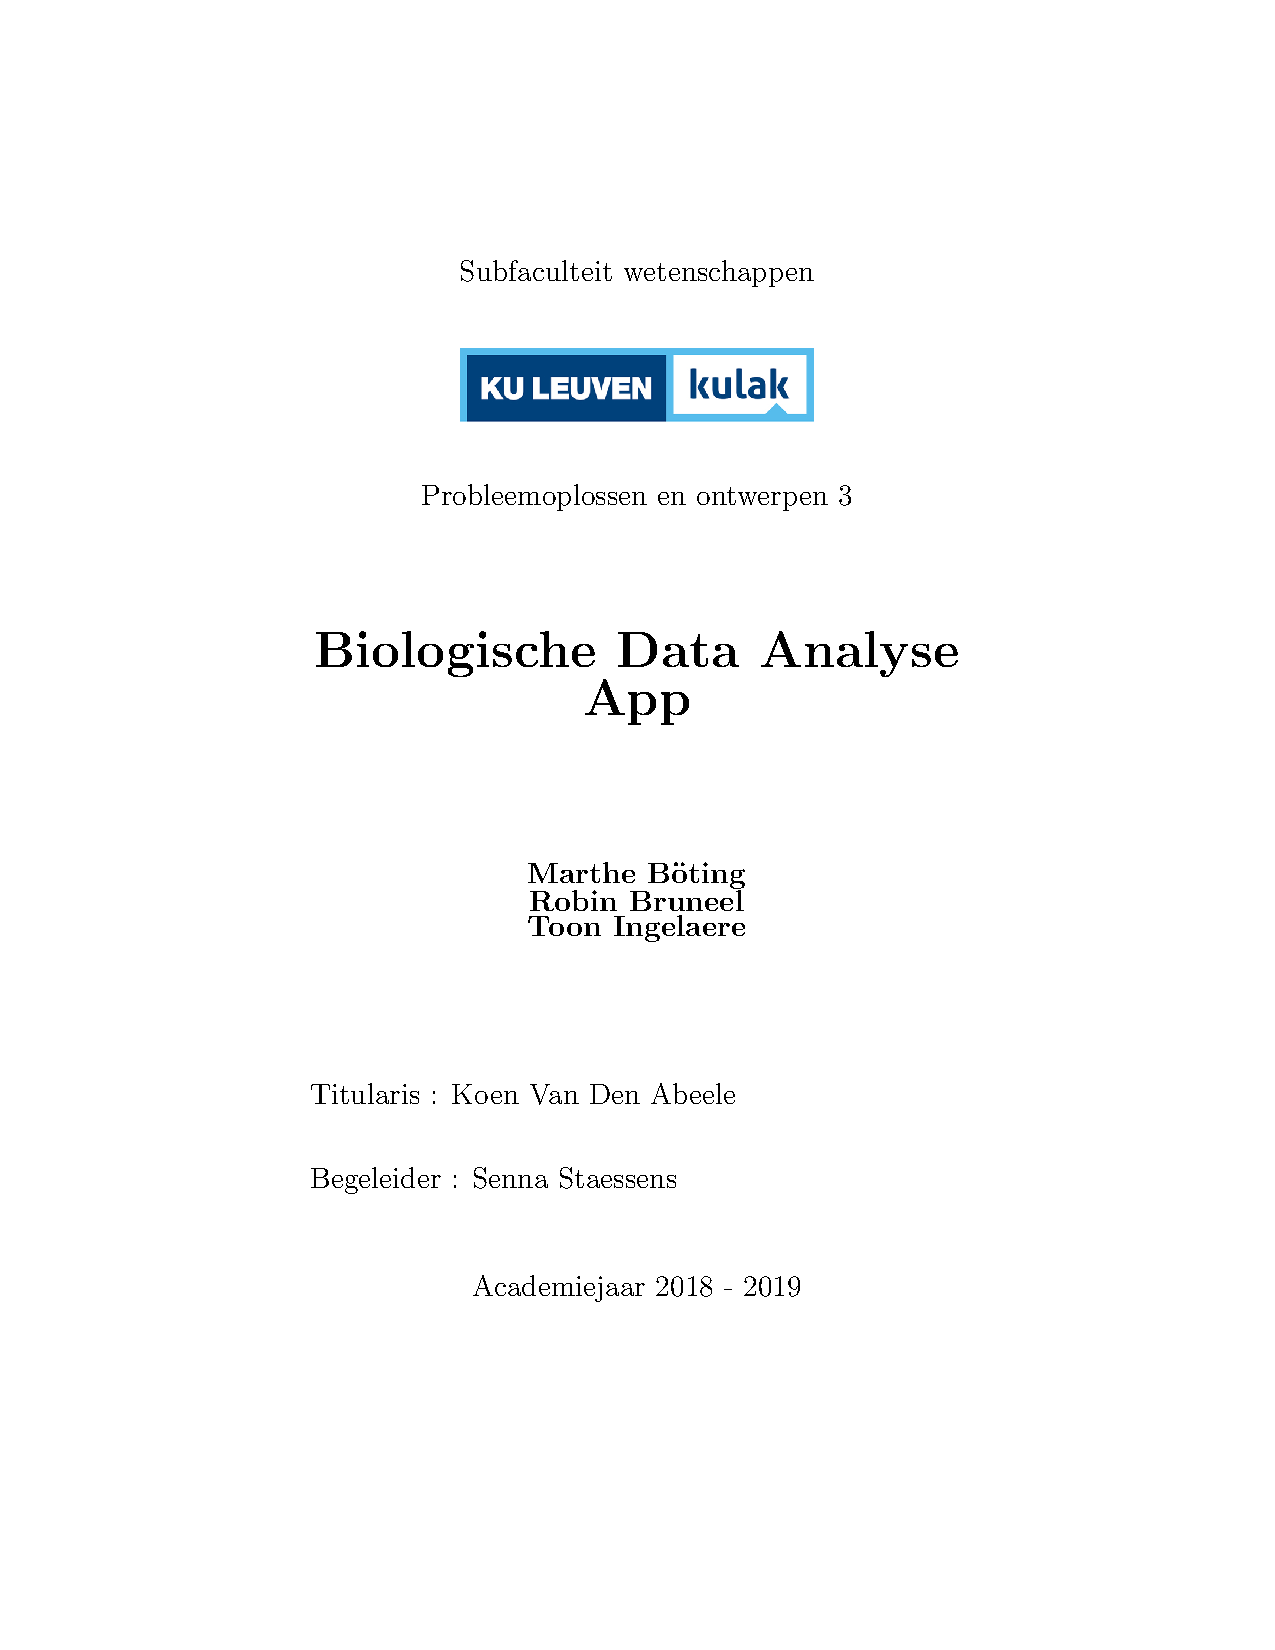
\includepdf{voorblad}
	
	\maketitle

\section*{Inleiding}

Inleidende tekst.

\tableofcontents

\section{ISectie-titel}


Tekst.

\section{De gebruiksvriendelijke applicatie}
De app werkt op basis van de klant die een foto kan ingeven. Het resultaat is een bewerkte foto waarbij er een percentage van de hoeveelheid aanwezig kleur weergegeven wordt.\\
Op het moment dat de klant een afbeelding gekozen heeft, zal  in de eerste fase de achtergrond van de foto wit worden gemaakt en wordt de foto bijgesneden zodanig dat enkel de bloedklonter zichtbaar is. Als dit gebeurd is, zal er al een eerste resultaat getoond worden. Hierdoor heeft de klant een beeld waarop de verdere analyse zal gebeuren en kan die eventueel ingrijpen bij fouten. \\
Vervolgens zal de kleurenanalyse gebeuren. Ook hiervoor zal de foto getoond worden waarop de klant kan zien welke delen de indicator bevatten en zal het percentage gegeven worden. \\
Soms is de kleuring intenser dan anders dit is het gevolg van verschillende factoren (bijvoorbeeld: temperatuur, druk, vochtigheid,... ). Hierdoor kan het resultaat die wordt bekomen via de app eens afwijken van de werkelijke waarde. Daarom hebben wij sliders toegevoegd. Zoals eerder vermeld hebben wij experimenteel waarden bepaald waartussen gewerkt wordt. Door het toevoegen van deze sliders kan de klant zelf deze waarden aanpassen wanneer de kleuring afwijkt. Deze kunnen ook gebruikt worden op het moment dat de bewerkte foto .
Daarnaast is er de mogelijkheid aan om niet foto per foto in te geven maar een volledige map met foto's die dan elk afzonderlijk bewerkt en opgeslagen worden.

\section*{Besluit}

Afsluitende tekst

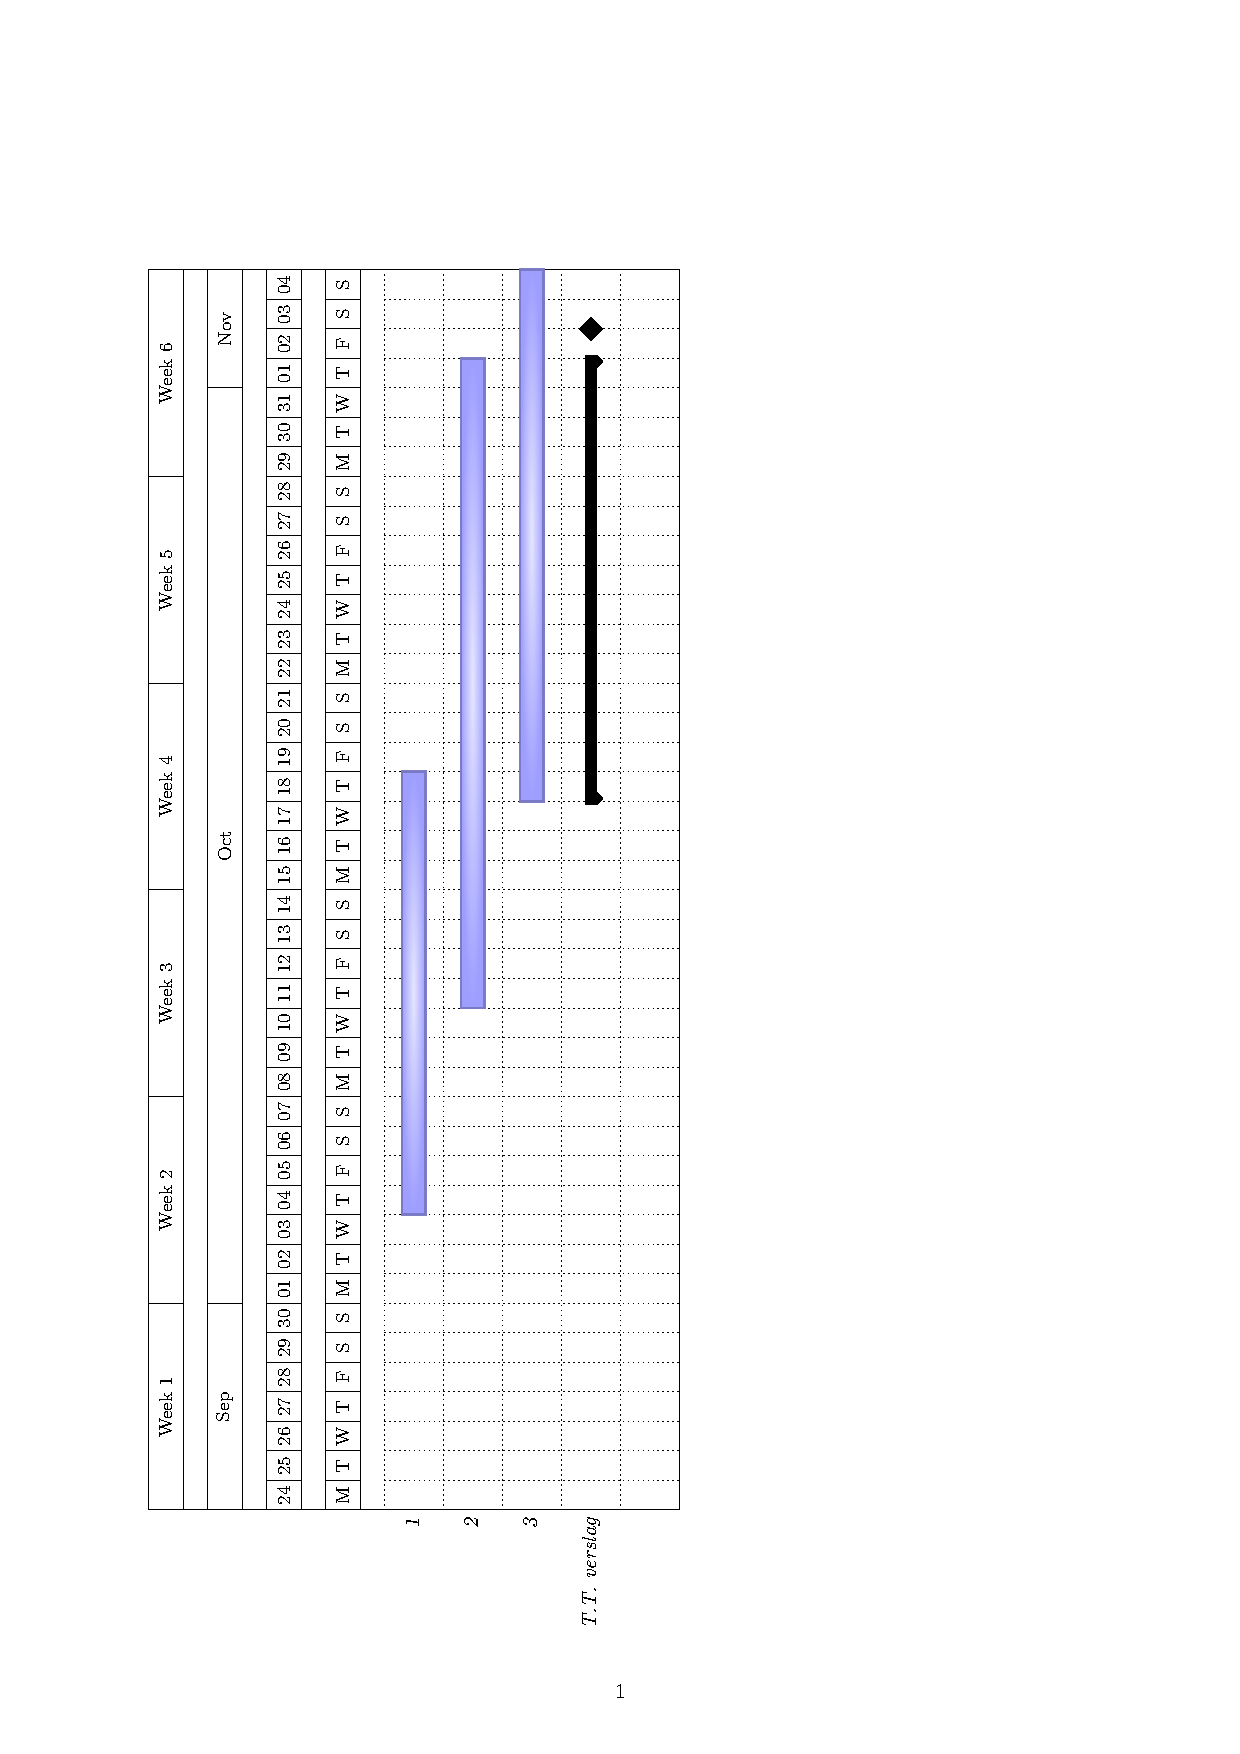
\includepdf[pages={1-3}]{ganttchart}

\end{document}
